\documentclass{article}[12pt;letterpaper]
\usepackage{graphicx}
\usepackage{verbatim}
\usepackage{color}
\usepackage[nohead,nofoot,left=1in,right=1in,top=1in,bottom=1in]{geometry}

\pagestyle{empty}
\raggedright
\frenchspacing
\setlength{\parskip}{0in}
\setlength{\parindent}{0in}

\newcommand{\todo}[1]{\textcolor{red}{TODO #1}}

\begin{document}

\begin{flushleft}
Parry Wilcox \\
Andrew Shen
\end{flushleft}

\section{Thread count scaling}

We ran \texttt{nbody -s 1352723313 -nt \$NTHREADS} for \texttt{\$NTHREADS = 1,
2, 4, 8}. For the most part we see the speedup that we expect from using more
threads:

\begin{tabular}{c l}
Thread Count & Time (s) \\
\hline{}
1 & 4.138442 \\
2 & 1.048486 \\
4 & 0.539792 \\
\end{tabular}

For eight cores, we saw some unusual behavior. For most runs, we observed a
slight decrease in performance with the correct results:

\begin{tabular}{l l l l l l l l}
0.559210 & 0.553203 & 0.573746 & 0.564950 &
0.581025 & 0.562103 & 0.562194 & 0.545826
\end{tabular}

But for some runs, particularly immediately consecutive runs, we saw that not
only did the performance decrease, but the integrity of the results was also
compromised:

\begin{verbatim}
###### 4 threads 

dt: 0.0005
Simulation box size: 0.715542
Random seed is 1352723313
# particles : 1024
Using static BLOCK decomposition
Nsteps: 1000

n = 1024, nsteps = 1000
(u,vMax) = ( 9.99816007e-01, 9.97788041e-01 )
(u,vL2 ) = ( 5.74424367e-01, 5.76119911e-01 )
Running time = 5.39792000e-01 sec.

###### 8 threads 

dt: 0.0005
Simulation box size: 0.715542
Random seed is 1352723313
# particles : 1024
Using static BLOCK decomposition
Nsteps: 1000

n = 1024, nsteps = 1000
(u,vMax) = ( 3.49390795e+03, 1.23453369e+04 )
(u,vL2 ) = ( 1.09315048e+02, 3.85857235e+02 )
Running time = 5.44501000e-01 sec.
\end{verbatim}

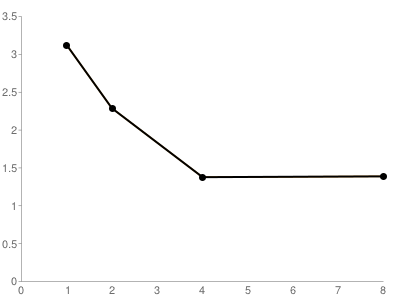
\includegraphics[width=0.3in]{a2_sec1_1.png}

We get a similar result when we use the \texttt{-b} flag for irregular
particle distribution (\texttt{nbody -b -s 1352723313 -nt \$NTHREADS}):

\begin{tabular}{c l}
Thread count & Time (s) \\
\hline{}
1 & 3.120088 \\
2 & \textcolor{red}{segmentation fault} \\ % FIXME!
4 & 0.175171 \\
8 & 0.351271
\end{tabular}

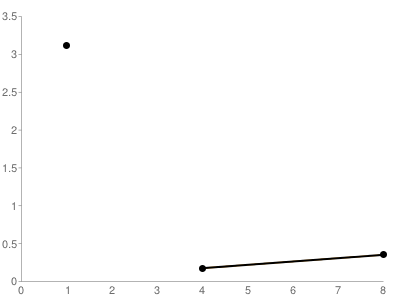
\includegraphics[width=0.3in]{a2_sec1_2.png}

\section{Chunk-scheduled scaling}

We ran \texttt{nbody -b -nt 8 -s 1352723313 -c \$CHUNKS} for \texttt{\$CHUNKS =
1, 2, 4, 8, 16, 32, 64, 128, 256, 512}. We notice that as the chunk size goes
to the number of particles, the load becomes imbalanced because only the first
few threads receive chunks to work on, causing a decrease in performance to a
level comparable to block partitioning with one thread.

\textit{Note: this was taken with load imbalancing removed. Maybe we should
get this data again?}

\begin{tabular}{c l}
Chunk size & Time (s) \\
\hline{}
  1 & 1.561923 \\
  2 & 1.433125 \\
  4 & 1.672107 \\
  8 & 1.546027 \\
 16 & 1.402706 \\
 32 & 1.482828 \\
 64 & 1.540522 \\
128 & 1.711720 \\
256 & 2.115562 \\
512 & 3.067487
\end{tabular}

% http://chart.apis.google.com/chart?cht=lxy&chs=400x300&chma=16,16,16,16&chxt=x,y&chxr=0,0,9|1,0,3.5,0.5&chds=0,9,0,3.5&chd=t:0,1,2,3,4,5,6,7,8,9|1.561923,1.433125,1.672107,1.546027,1.402706,1.482828,1.540522,1.71172,2.115562,3.067487&chm=D,000000,0,0,2|o,000000,0,,5&chxl=0:|1|2|4|8|16|32|64|128|256|512
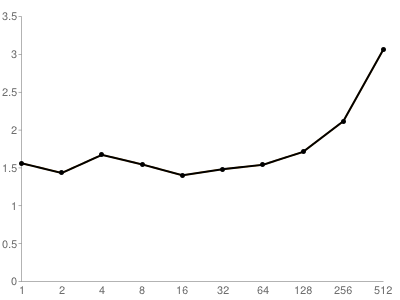
\includegraphics[width=0.3in]{a2_sec2_1.png}

A similar effect appears without load imbalancing.

\begin{tabular}{c l}
Chunk size & Time (s) \\
\hline{}
   1 & 1.702923 \\
   2 & 1.609537 \\
   4 & 1.602867 \\
   8 & 1.522705 \\
  16 & 1.568501 \\
  32 & 1.628063 \\
  64 & 1.669489 \\
 128 & 1.643170 \\
 256 & 2.191104 \\
 512 & 3.044322 \\
1024 & 5.023962
\end{tabular}

% http://chart.apis.google.com/chart?cht=lxy&chs=400x300&chma=16,16,16,16&chxt=x,y&chxr=0,0,10|1,0,6&chds=0,10,0,6&chd=t:0,1,2,3,4,5,6,7,8,9,10|1.702923,1.609537,1.602867,1.522705,1.568501,1.628063,1.669489,1.64317,2.191104,3.044322,5.023962&chm=D,000000,0,0,2|o,000000,0,,5&chxl=0:|1|2|4|8|16|32|64|128|256|512|1024
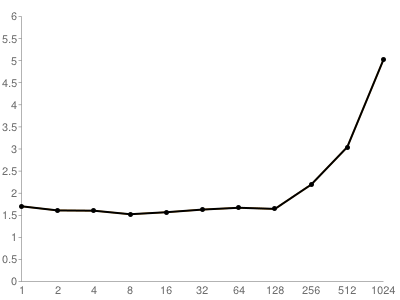
\includegraphics[width=0.3]{a2_sec2_2.png}

\section{Comparison of block and chunk partitioning}

We ran block and chunk (size 4) partitioning for each allowed number of threads
(1, 2, 4, 8). There is a comparable speedup between both methods. This is
probably because having the correct chunk size allows dynamic scheduling to
more evenly distribute small blocks of work among workers, so that the speedup
is comparable to the speedup that we get from just throwing more processors at
the problem.

\begin{tabular}{c l l}
Thread count & Block time (s) & Chunk=4 time (s) \\
\hline{}
1 & 4.162895 & 4.175521 \\
2 & 2.362130 & 2.401542 \\
4 & 1.576841 & 1.557133 \\
8 & 1.592611 & 1.588439
\end{tabular}

We disabled load imbalancing, so we could not take measurements for it.

\section{Performance bottlenecks}

We notice that a lot of time is spent idling at barriers in each thread. This
is probably a consequence of the extremely conservative way in which we
implemented coherence, which needed barriers after every parallel computation
and after every reset of the counter that we used for dynamic chunk scheduling.

We also had problems with data races. \todo{Parry please help me explain this.}

\end{document}
